\chapter{Implementing policy-agnostic programming on the client side\label{chap:solution}}
We incorporated policy-agnostic programming into Javascript by adding constructs
defined for the Jeeves language as a subsystem. We chose Narcissus~\cite{narc},
a Javascript interpreter written in Javascript, to create the proof of concept.
Narcissus was built by its developers to be able to prototype new language features
for Javascript.

\section{Implementing faceted values in Narcissus}
Integral to implementing Jeeves is the implementation of faceted values. Our implementation
of faceted values derives heavily from the work done by Austin and Flanagan~\cite{Faceted}
and is inspired from the concept presented by Kerchove et al~\cite{Modular} for
``modular instrumentation'' of interpreters. They talk about how many dynamic analysis
approaches for information flow security have prototypes that are implemented in
very specific ways making it difficult to compare and reuse. They derive some
specific criteria to follow in order to achieve ``modular instrumentation'' using
the implementation of~\cite{Faceted} as a case study. While we borrow a few ideas
from this, our implementation does not follow the criteria specified because achieving
``modular instrumentation'' would involve non-trivial changes to the Narcissus
interpreter making it out of scope of our problem. What we did achieve is untangling
of the concerns of the core interpreter for non-faceted evaluation from the concerns
of faceted evaluation. This makes it easier to relate principles of faceted evaluation
with the implemented prototype and also to extend or reuse it.

Our implementation of faceted values is independent from the core Narcissus interpreter.
This involved making the core interpreter modular to be able to modify existing
evaluation mechanisms to behave differently for faceted values. The Narcissus interpreter
has an execute function which consists a switch case control flow that is set to
perform the appropriate set of operations based on the type of node identified by
the parser. Wherever there is need for faceted behavior, instead of making the core
interpreter code handle faceted behavior, we moved the part we would need to change
into a method and later override the method to handle faceted behavior.
Figure~\ref{fig:facetif} shows how this overriding is implemented for the [F-IF-SPLIT]
evaluation rule. Here, \texttt{BaseExecContext} is an object that stores a copy of all the
methods from the core interpreter which we need to override. \texttt{ExecutionContext}
is an object from the core interpreter that keeps track of the current flow of execution.
\texttt{FacetExecContext} is the \texttt{ExecutionContext} object extended with
the \textit{pc} to help keep track of the influence of public or private facets
on the current flow of execution. In the \texttt{evalIfBlock} function, notice we
call the base \texttt{evalIfBlock} function if \texttt{cond} is not a faceted value.
Otherwise, we call the \texttt{evaluateEach} function which encapsulates all the
function application rules from Figure\ref{fig:appRules}. Similarly, we have built
the rest of the functions in \texttt{BaseExecContext}.
\lstset{
  language=javascript,
  frame=single,
  breaklines=true,
  basicstyle=\footnotesize\ttfamily,
  numbers=left,
  extendedchars=true,
  tabsize=2
}
\begin{figure}
  \begin{lstlisting}
/**
 * Preserving original behavior of these functions
 */
var BaseExecContext = {
  getValue: interpreter.ExecutionContext.prototype.getValue,
  putValue: interpreter.ExecutionContext.prototype.putValue,
  evalBinOp: interpreter.ExecutionContext.prototype.evalBinOp,
  evalUnaryOp: interpreter.ExecutionContext.prototype.evalUnaryOp,
  evalIfBlock: interpreter.ExecutionContext.prototype.evalIfBlock
};

/**
 * If block behavior when condition is faceted
 *
 * @param cond
 * @param thenPart
 * @param elsePart
 */
FacetExecContext.prototype.evalIfBlock = function(cond,thenPart,elsePart) {
  var execContext = FacetExecContext.current;
  if (cond instanceof FacetedValue) {
    evaluateEach(cond, function(v, x) {
      if (v) {
        interpreter.execute(thenPart, x);
      } else if (elsePart) {
        interpreter.execute(elsePart, x);
      }
    }, execContext);
  } else {
    BaseExecContext.evalIfBlock.call(this,cond,thenPart,elsePart);
  }
};
  \end{lstlisting}
  \caption{Independent implementation of faceted behavior for the ``if'' control flow}
  \label{fig:facetif}
\end{figure}

\begin{figure}
  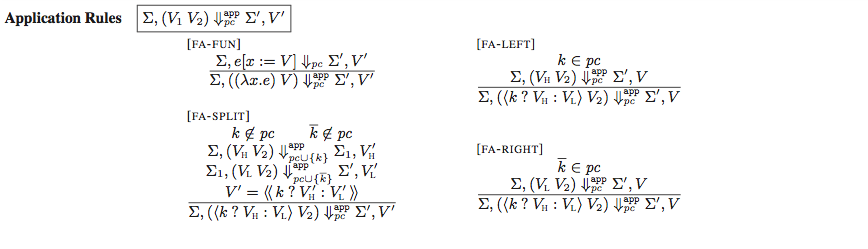
\includegraphics[scale=0.5, frame]{images/appRules}
  \caption{Function application rules~\cite{FacetedJeeves}}
  \label{fig:appRules}
\end{figure}

\section{Implementing Jeeves}
Once we had faceted values working, adding support for Jeeves constructs was pretty
straightforward. All of the Jeeves constructs are encapsulated in the \texttt{PolicyEnvironment}
prototype.
